\documentclass[journal,12pt,twocolumn]{IEEEtran}

\usepackage{enumitem}
\usepackage{amsmath}
\usepackage{amssymb}
\usepackage{graphicx}


\title{Assignment 2 \\}
\author{Suryaansh Jain \\ \normalsize cs21btech11057 \\}


\begin{document}
	% The title
	\maketitle
	
	% The question
	\textbf{Question 21(a)} 
	A product can be manufactured at a total cost $C(x) = \frac{x^{2}}{100}+100x+40$, where x
is the number of units produced. The price at which each unit can be sold is given
by $P$ = $200 - \frac{x}{400}$. Determine the production level x at which the profit is
maximum. What is the price per unit and total profit at the level of production? \\
	
	
	% The solution
	\textbf{Solution.}		
	\begin{align}
	    &\text{Let\ the\ total\ price\ }p(x) = P.x \\
		&\implies \frac{p(x)}{x} = 200 - \frac{x}{400} \\
		&c(x) = \frac{x^{2}}{100} + 100x + 40 \\
		&Profit = p(x) - c(x)
	\end{align}
	
	For maximum profit $\frac{dProfit}{dx} = 0$
	
	\begin{align}
	    &\implies 100 - \frac{x}{40} = 0 \\
	    &\implies x = 4000
	\end{align}
	
	The total production level $x = 4000$.
	
	\begin{align}
        &Price\ per\ unit =  \frac{c(x)}{x}  = 190 \\
        &p(x)= 199960
	\end{align}
	
	Total profit = 199960
			
	
	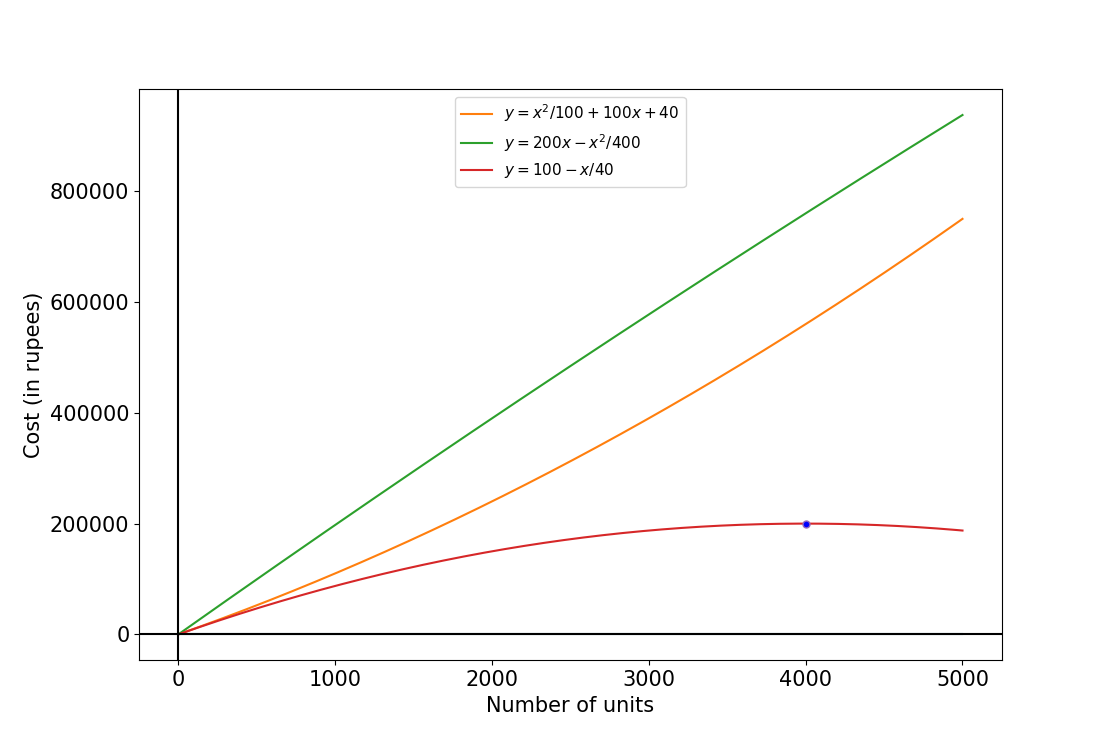
\includegraphics[scale = 0.25]{main.png}
	
\end{document}
